\documentclass[12pt]{amsart}
\usepackage[fullpage]{geometry}
\usepackage{fullpage}
\usepackage{pbox}
\usepackage{graphicx}
\usepackage{booktabs} % Top and bottom rules for table
\usepackage{amsfonts, amsmath, amsthm, amssymb}
\usepackage{longtable,array,color,xcolor}
\usepackage[colorlinks = true,
            urlcolor  = blue]{hyperref}
\usepackage{verbatim}
\usepackage{enumerate}
\newcommand\narrowstyle{\SetTracking{encoding=*}{-50}\lsstyle}

\setlength{\parindent}{0pt}

\begin{document}

\title{Math 320: Homework 3}
Due: September 30, 2016
\maketitle

Please read through chapters 5 and 6 in the textbook.
Answer the following questions. Please submit all code
and output with brief descriptions of what you are doing.

\vspace{5mm}

\begin{enumerate}

\item {\em Solution:} \begin{enumerate}[(a)]
\item The following code works as a {\tt falsi} MATLAB function:
\begin{verbatim}
function approx = falsi(l,r,func,epsilon,maxSteps)
%INPUT: a function func, with bracket [l,r], a.r.e. bound epsilon,
% and maximum step number maxSteps.
%OUTPUT: a point approx giving the x-value of the most
%recent approximation to the root.
new = l;
old = r;
iterCount = 0;
while (abs(r - l) > 2*epsilon) & ... 
        (iterCount <= maxSteps)
    %Compute y-values for endpoints
    old = new;
    fl= func(l); fr = func(r);
    %Compute linear interpolation point and y-value
    new = l - fl*(r-l)/(fr- fl);
    val = func(new);
    %Redefine your bracket based on the sign.
    if sign(val) == sign(fl)
        l = new;
    elseif sign(val) == sign(fr)
        r = new;
    end
    %exit the loop if the a.r.e. is small enough.
    if ((new - old)/new <= epsilon)
        break
    end
    %Step up the count of iterations.
    iterCount = iterCount + 1;
end
approx = new;
end

\end{verbatim}

\item The value output by MATLAB after 18 iterations is
2.030525784672327. (Use {\tt format long} to obtain this
level of precision.)

\item There are a few ways to go about this. I added an
optional argument ``root'' to the {\tt falsi} function,
and included these lines of code before the while loop:
\begin{verbatim}
if nargin == 6
    truerr = [];
    apperr = [];
end
\end{verbatim}

Then, inside of the while loop, I included these lines of code:
\begin{verbatim}
if nargin == 6
    truerr = [truerr [abs(new - rt)/rt]];
    apperr = [apperr [abs(new - old)/old]];
end
\end{verbatim}

After obtaining the sequences of errors. I plotted them
using the following code: {\tt semilogy(1:18,t,'o-',2:18,a(2:18),'-*')}.

\begin{figure}[h!]
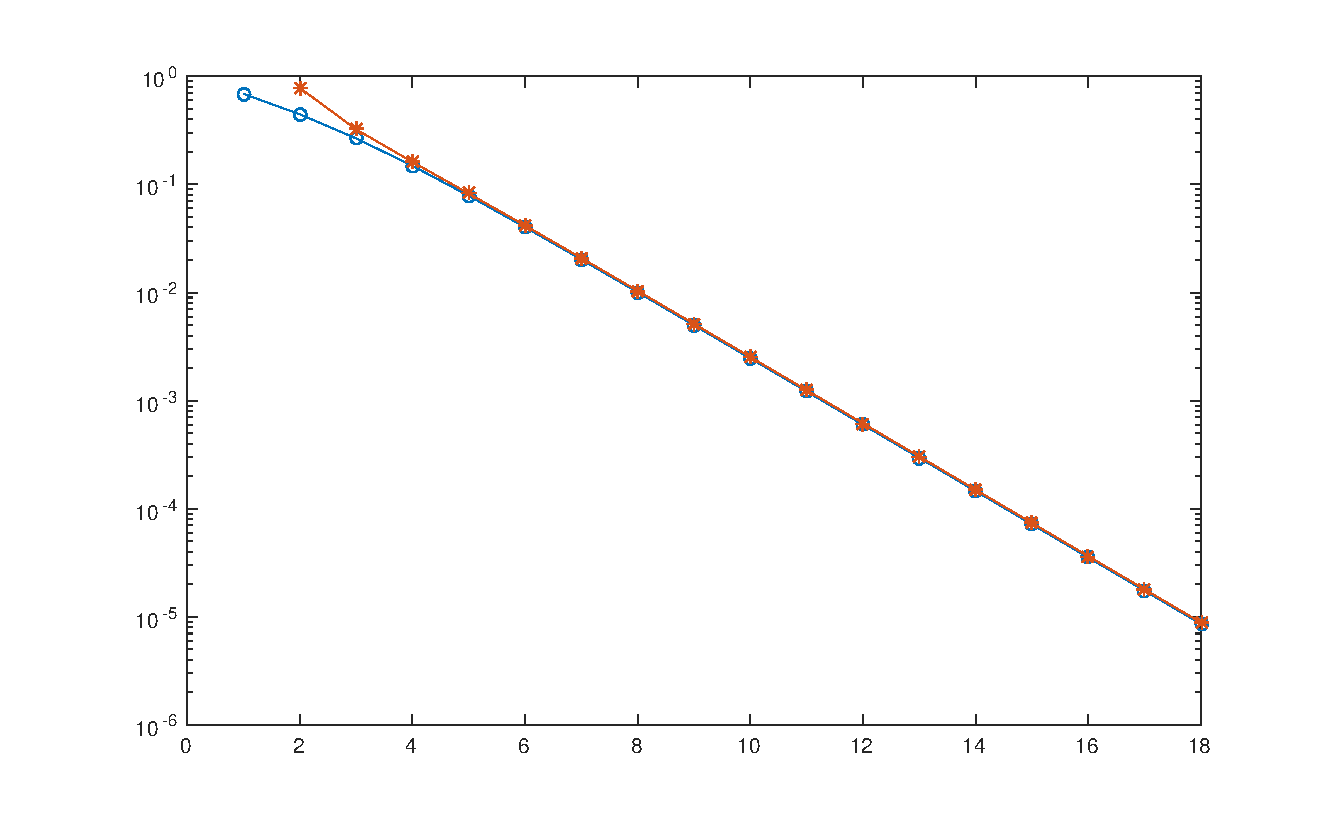
\includegraphics[width=\textwidth]{hw3fig1.eps}
\end{figure}
\end{enumerate}
\item {\em Solution:}
\begin{enumerate}
\item The following code works for implementing the secant
method.
\begin{verbatim}
function approx = secant(x0,x1,func,epsilon,maxSteps)
%INPUT: a function func, with two approximations, 
%a.r.e. bound epsilon, and maximum step number maxSteps.
%OUTPUT: a point approx giving the x-value of the most
%recent approximation to the root.
new = x1;
old = x0;
iterCount = 0;

while (iterCount <= maxSteps)
    %Step up the count of iterations.    
    iterCount = iterCount + 1;
    %Compute y-values for two points
    f1= func(new); f2 = func(old);
    %Compute linear interpolation point and y-value
    mid = new - f1*(new-old)/(f1 - f2);
    old = new;
    new = mid;
    %exit the loop if the a.r.e. is small enough.
    if (abs(new - old)/new <= epsilon)
        break
    end
end
approx = new;
end
\end{verbatim}

\vspace{3mm}

\item The value output by MATLAB after 7 iterations is
4.536403654894378.

\vspace{3mm}

\item  The value output by MATLAB after 7 iterations is 
1.857183860152164.
\vspace{3mm}

\item There are also a number of ways to do this. I used
the following command to initialize a collection of points:
{\tt pts = [old new];} and then the following code inside the 
loop to collect points: {\tt pts = [pts new];}

After the loop is complete we carry out the plots using the
following sequence of commands:

\begin{verbatim}
X = linspace(min(pts)-.1,max(pts)+.1,500);
Y = arrayfun(func, X);
plot(X,Y,'-k');
hold on
plot(X,zeros(1,500),'-k');
fpts = arrayfun(func, pts);
for i=3:length(pts)
    plot(pts(i-2:i),[fpts(i-2),fpts(i-1),0],'r')
    plot([pts(i),pts(i)],[0,fpts(i)],'--b')
end
axis([min(X),max(X),min(Y),max(Y)]);
\end{verbatim}

\vspace{5mm}

The output for our two plots is here:

\begin{tabular}{c}
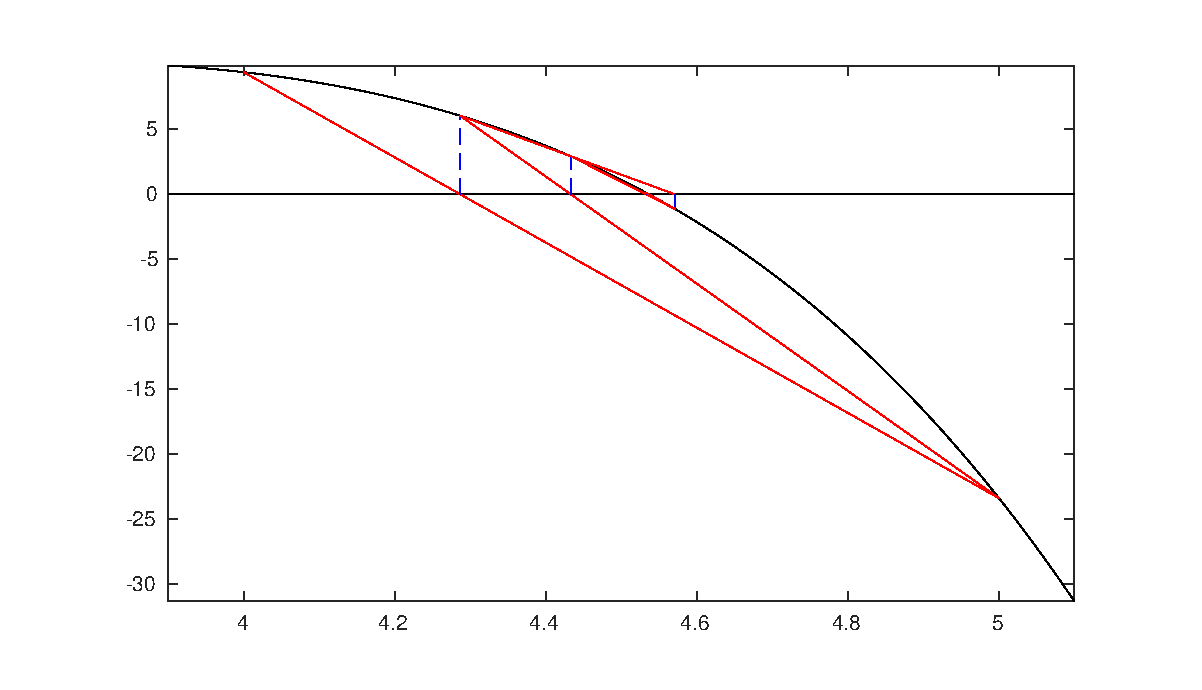
\includegraphics[width=.8\textwidth]{hw3fig3.eps} \\
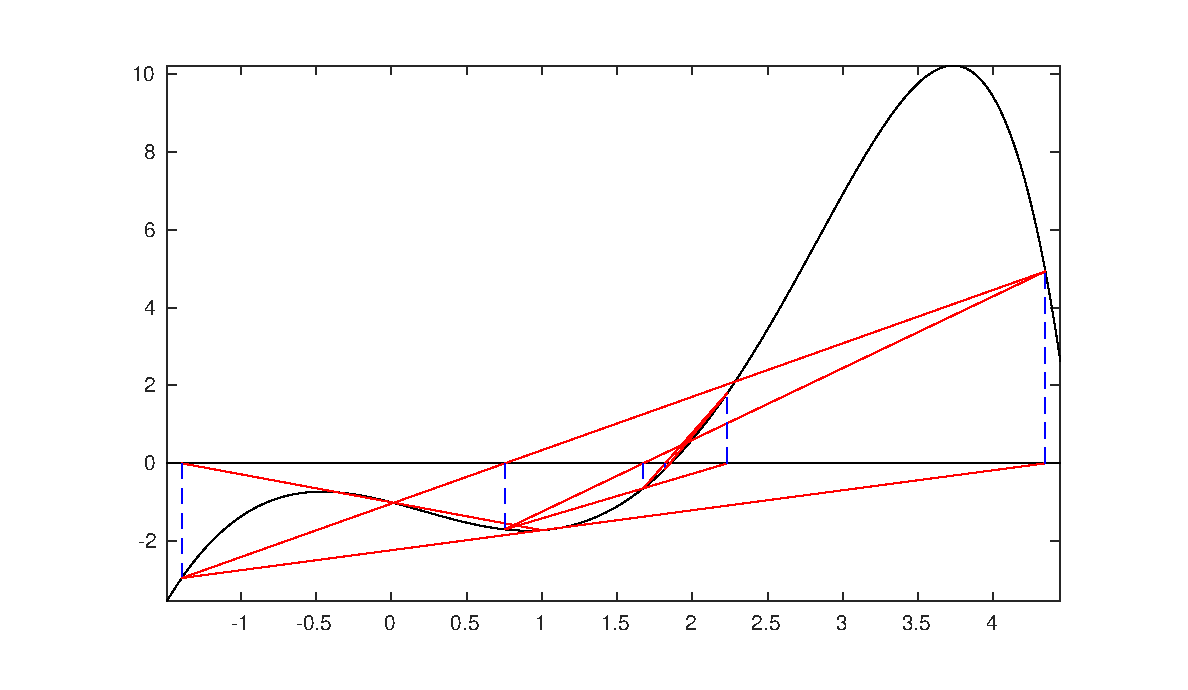
\includegraphics[width=.8\textwidth]{hw3fig2.eps} \end{tabular}
\end{enumerate}

%\vfill
%\pagebreak

\item Let $E_n = x_n - r$. We claim that $\lim_{n \to \infty} E_n/ E_{n-1}^2 = \mu$.

The formula for $x_n = x_{n-1} - f(x_{n-1})/f'(x_{n-1})$. Because the function
is smooth, and the root is simple, we can use Taylor's theorem
to write $f(x_n) = f(r) +$ \\ $f'(r)(x_n-r) + \frac{1}{2}f''(\xi)(x_n - r)^2$ where $\xi$ is between $r$ and $x_n$ and $f'(r)$ is nonzero.

Using this expansion, we have:
\[ E_n = E_{n-1} - \dfrac{f'(r)E_{n-1} + \frac{1}{2} f''(\xi)E_{n-1}^2}{f'(r) +  f''(\xi)E_{n-1} }\]
\[ E_n = \dfrac{E_{n-1}(f'(r) +  f''(\xi)E_{n-1} )}{f'(r) +  f''(\xi)E_{n-1} } - \dfrac{f'(r)E_{n-1} + \frac{1}{2} f''(\xi)E_{n-1}^2}{f'(r) +  f''(\xi)E_{n-1} }\]
\[ E_n = \dfrac{\frac{1}{2} f''(\xi)E_{n-1}^2}{f'(r) +  f''(\xi)E_{n-1} }\]

\[ E_n/E_{n-1}^2 = \frac{1}{2}f''(\xi)\dfrac{1}{f'(r) + f''(\xi)E_{n-1}}\]

The limit of the expression on the right as $n\to \infty$ is finite
since $f'(r) \neq 0$.
\vspace{1cm}

\item 
\begin{itemize}
\item Bisection Method for $f(x)$. This method will not find the root,
since the values on either side of it are nonnegative.
\item Incremental Search Method for $f'(x)$. This method 
can find a collection of intervals where the root might be. Since $f(l)$
and $f(r)$ are presumably greater than $0$ (if not, then we found the root),
the Mean Value Theorem implies that the derivative is negative at
some point before the root, and positive at some point after the root. The
incremental search will find an interval where it's zero.
\item Newton's Method. This method should converge to the root, but
slower than if it were a simple root. Consider the example of the parabola
$x^2$.  Any point $x_n$ nearby points to $x_{n+1} = x_n - x_n/2$. This
clearly points towards zero.
\item Secant Method. This method should also converge to the root; like
Newton's method, it will converge more slowly than usual. Here, too, consider
the parabola $f(x) = x^2$ and begin with points within $1/2$ of zero. Then
$x_{n+1} = x_n -x_n^2 \dfrac{x_n^2 - x_{n-1}^2}{x_n - x_{n-1}} = x_n - x_n^2(x_n + x_{n-1})$.
Assuming $0 < x_n, x_{n-1} < 1/2$, the subtracted term will be less than $x_n$ meaning
that it moves towards zero without overshooting.
\end{itemize}

\end{enumerate}


\end{document}
